\section{Sensitivity to Error Surface Quality}
In the spirit of the list above provided by \cite{van2007neurofitter}, the next item should be called ``Efficient Convergence", but this efficiency really comes down to the nature of the error surface created by the choice of models, tests, and experimental data.

\subsection{Objective Function Dimensionality vs Model Parameter Dimensionality}
If a given class of models is capable of describing the behavior of a given real neuron, then the number of independent, reliable tests used to generate the objective function can be as large as desired; more tests just provide more information to quickly rule out irrelevant regions of parameter space.
On the other hand if a model class is only capable of describing a fraction of the real neuron's behavior, too many distinct tests will result in an optimization problem that can never be fully satisfied.
Since ``all models are wrong, but some are useful" (Box, 1976), let us imagine that we usually in the latter case.

\subsection{When Does Genetic Optimization Get Stuck?}
Genetic algorithms are known as derivative-free optimizers, since they do not follow any gradient down the error surface, or even know of the existence of such a gradient.
Chromosomes only survive and reproduce differentially according to their location on the error surface.
Thus, genetic optimization is never truly "stuck" inside a local minima on the error surface, as mutation or crossover can always produce new chromosomes outside the basin of attraction.
Despite this robustness, just like in gradient descent, genetic algorithms can only be guided by information in the error surface.
When the objective function has a low-dimensionality, for example when it is based upon tests that mostly compute small variations on the same small number of features of the simulation output, it may not provide enough information to distinguish one location in parameter space from another one close by, even though the first may be closer to the optimal solution than the second.
In other words, many regions of parameter space may be locally flat at a mesoscopic scale, and local minima at a microscopic scale may thus be difficult to escape.
No lower error solution may be available within a reasonable distance (in parameter space) from the current one.

\subsection{Defects in the Error Surface}
The real error surfaces that guide optimization here have ``defects", for example discontinuities (due perhaps to bifurcations in the underlying dynamical system, e.g. from spiking to non-spiking) or to deep local minima, that make optimization challenging.
I coined the term "corrugated" to describe surfaces low amplitude oscillatory disturbances across the error surface.

Some optimization techniques require a perfectly convex error surface to converge.
Genetic algorithms are more tolerant, up to a point, but an extremely high dimensional optimization problem with a large number of optima can still be intractable.
So which error surface defects are truly harmful?.
This largely comes down to scale.
The corrugation observed in the error surfaces here was typically on a much smaller scale than the long-range structure that guides optimization.
Consider something analogous to a signal-to-noise ratio (SNR), describing the information that guides optimization vs the wrinkles that impede it.
When SNR is larger, defects are less consequential.

I observed that the NSGA2 selection algorithm was particular vulnerable to defects in the error surface, and required a higher SNR to obtain optimal solutions.
NSGA2 is a fundamentally conservative and short-range approach to evolution, so it may simply lack the drive to escape problematic regions of the error surface.
Unlike NSGA2, IBEA was less sensitive to such defects, and required a lower SNR to converge rapidly. 

However, in any algorithm as the optimum is approached, the rate of mutation must slow down to enable efficient short-range exploitation of the peri-optimum region.
one should not expect to see evidence of efficient-learning. In later stages of This is precisely the phase when the optimizer will be more sensitive to small amplitude corrugations, which become large relative to the small gains to by moving between, say, a parameter set $1\%$ away from the optimum and the optimum itself.

The multiobjective function is derived from the objective functions associated with each feature used in optimization.
As such, the multiobjective function will be more corrugated if more of the component objective functions are corrugated.
Consequently, optimization is more likely to converge if the number of corrguated components is kept to a minimum.
In practice, I observed satisfactory solutions even when only $>\frac{1}{2}$ total number of objectives had no corrugation.
For example, in a four-objective problem, if the $4$th objective is uninformative, but not actively misleading, inclusion of that 4th objective may only slow down the speed of optimizer convergence, but not actually change the final outcome.
By contrast, if that $4th$ objective is actively misleading, the optimizer will likely find a satisfactory (but non-optimal) solution by compromising with the dominant $3$ objective functions.

\subsection{Examples of Challenging Neural Model Error Surfaces Encountered in This Work}
In the figures below, I describe the spectrum of error surface quality.
\begin{comment}
\begin{figure}
\begin{center}
     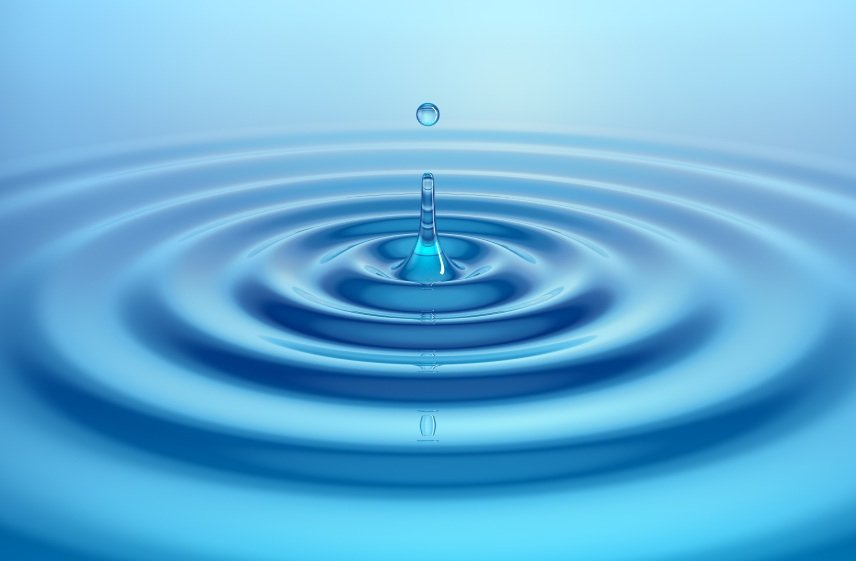
\includegraphics[scale=0.65]{figures/pond_ripple_surface.png}
     \caption[Conceptualizing moderate to worst case error surfaces]{In the case of pond ripples the cost function is defined so that the maxima is the optimal location on the surface. Ripples on a body of water are more challenging to optimize, as the water surfaces are approximately flat on the large scale, yet on the small scale maximas will be temporary preoccupy the GAs learning, but outside of those peaks, there is little large scale information to utilize.}
      
      \label{fig:test1}
\end{center}

\end{figure}
\end{comment}

\begin{figure}
      \centering
      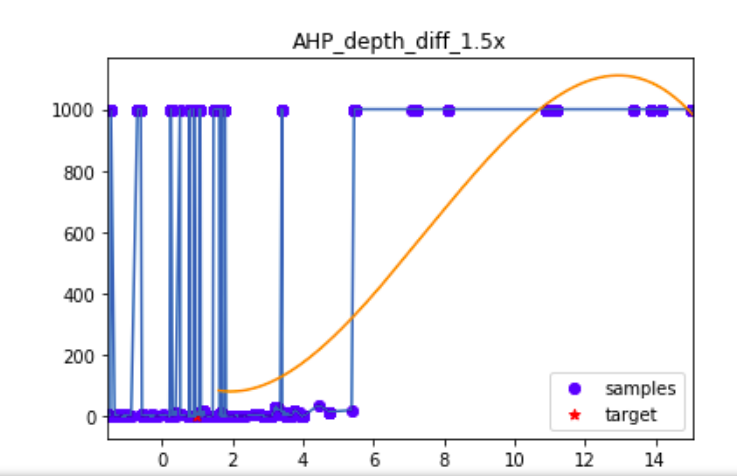
\includegraphics[scale=0.85]{figures/parameter_b_hopeless_surface2.png}
      \caption[Cross section of difficult or hopeless error surface]{Parameter b was slowly varied in the Izhikevich model while all other parameters where held constant, the AHP depth differences at $1.5 \times rheobase$, was computed for each different model parameterisation of \emph{a}, this resulted in a highly  discontinuous error surface, densely populated by local minima. A polynomial regression algorithm (orange trace) shows that if the error function is smoothed it looks convex, but it is very doubtfull that the GA would experience the error as anything but random}
      \label{fig:discontinuous_constraint}
\end{figure}


% Note Help wanted making a professional version, of this known to be unattractive draft/concept figure.
\begin{figure}
\centering
      \label{fig:test1}
      \centering
      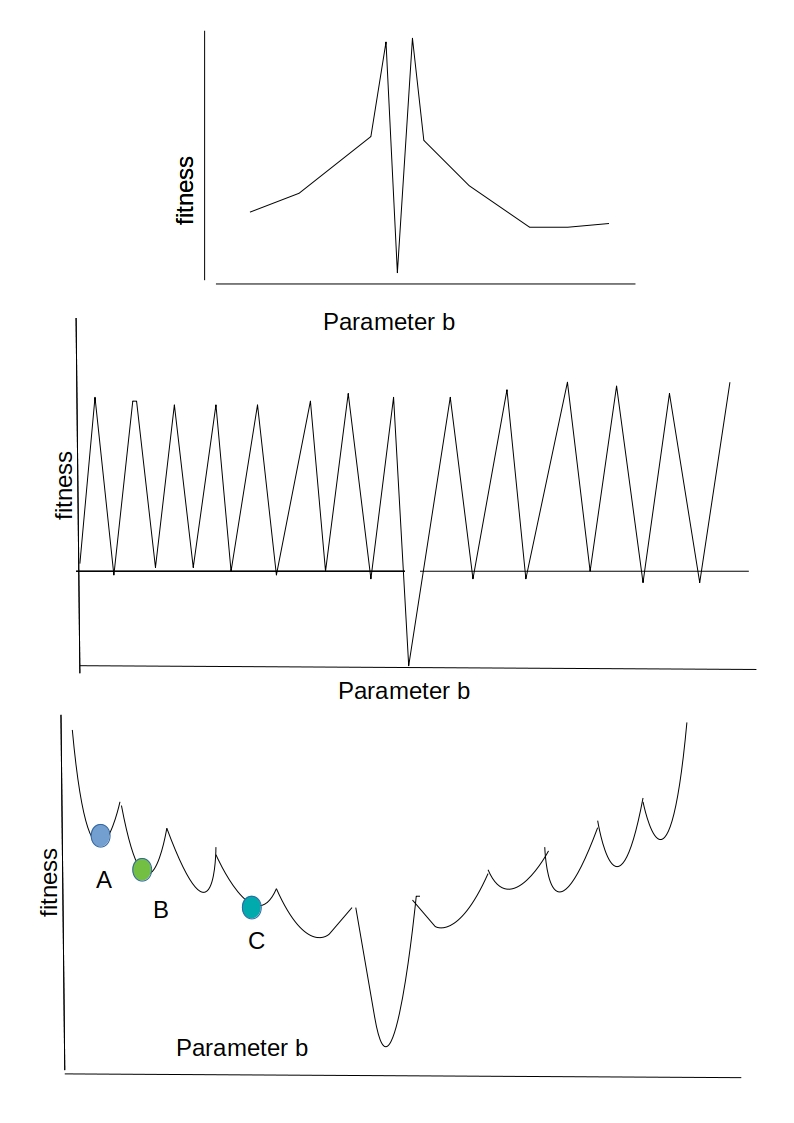
\includegraphics[scale=0.75]{figures/spectrum_worst_error_surfaces2.jpg}
      \caption[Hypothetical Error Functions, Worse than Rastrigrins function]{Rastrigrins function describes a challenging error surface, but one with learnable global features that a genetic algorithm can exploit. Consider the bottom inset figure, which is a cross section of a Rastrigin like function. Along the course of evolution, there is plenty of opportunity for genes like A and B to recombine, often producing fitter children like C. It's important to note that there are much worse error surfaces, and these may show up in practice consider for example the middle inset figure, where cross-over has nothing useful to contribute.
      The situation in the topmost inset is worse again still. In this context learning is a disadvantage, if the optimizer "learns", then it actually slows obtaining an optimal solution, which it will only find using an extremely lucky right large random mutation. It is likely that a GA on this surface will be slower than grid search.}
      \label{fig:test2}
\end{figure}      
      % The second type of error surface actually a 1D (and upside down) cross section of the 2D pond diagram, only actively misleads locally, globally it simply contains no helpful global information. Learning will not be of any assistance in obtaining the optima, but also learning won't be a disadvantage either, the Genetic Algorithm, will simply behave as a random sample testing algorithm, the GA will find the optimum in time, but possibly not as quickly or reliably as exhaustive search would. The second figure is a cross section of the pond ripple argument}


\begin{figure}
\centering
      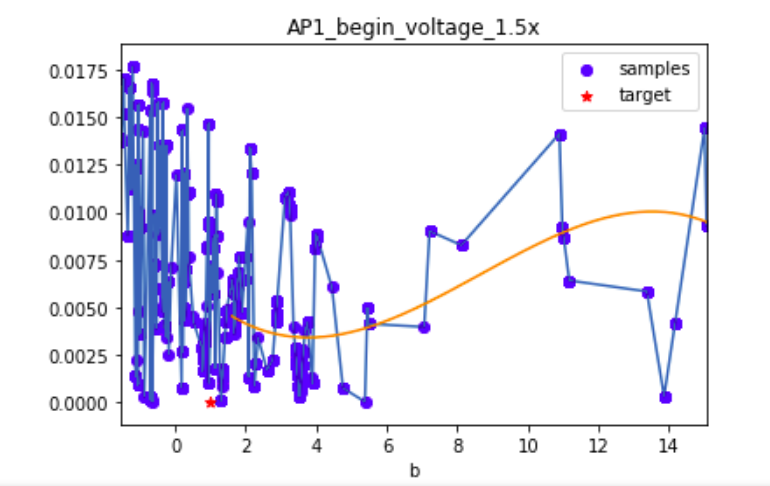
\includegraphics[scale=0.85]{figures/parameter_b_hopeless_surface.png}
      \caption[Cross section of an objective function that harms efficient optimization]{Parameter b was slowly varied in the Izhikevich model while all other parameters where held constant, the AP1 begin voltage (threshold), was computed for each different value of \emph{a} in the model. Evaluation of swept increments of \emph{a} resulted in the highly rippled error surface visible here. The surface is densely populated by local minima, and it lacks significant convex shape. A polynomial regression algorithm (orange trace), is a very bad fit of the error function. This implies that the function is not very smooth, and seemingly random. The optima value depicted as a red star. The optima is buried in random irregularities of error surface.
    }
      \label{fig:probably_smooth_constraint}
\end{figure}

\begin{figure}      
\centering
      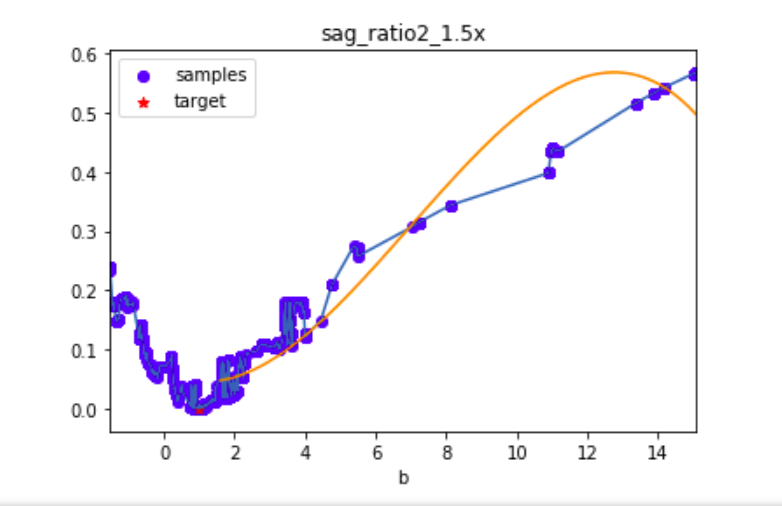
\includegraphics[scale=0.85]{figures/parameter_b_friendly_surface.png}
      \caption[Cross section of a more ideal objective function]{
      sag-ratio at 1.5 $\times$ rheobase error is plotted (y-axis) as I sweep across values of b $(x-axis)$. A polynomial regression algorithm (orange trace), is actually a semi reasonable fit of the error function. The quality of it fit entails smoothness.
    
    This is a cross section of a useable and tractable error surface, it has learnable global and local information, this surface is likely to be a valuable addition to the optimizer suite. The optima is depicted as a red star, but it is mainly superimposed by blue data points. The optima is find-able via using either the blue dots, or the orange regression lines as guides.}
      \label{fig:test2}
\end{figure}


%   When considering 2D relationships between single parameters and single objective functions, ideally each error function might contribute helpful information, which en-masse boosts the total amount of helpful information. For-instance some 2D error mappings, may contain one or more local minima, but in the same region a different error mapping could lack the error well, meaning that at least one out of two error functions contribute incentive to stride across a minima. The mapping that contains wells, might still be useful to guide optimization, as it may also lack minima in regions were the counterpart has them, additionally the alternative mapping may have regions of $~0.0$ gradient where the other mapping contains significant gradient.
   
   % I am not sure if its impossible to make progress.
 %  Through strategy it is possible to optimize satisfactorily without complete prior knowledge of error surfaces, although such a strategy is not recommended. If prior knowledge of an error surface is prohibited, evolutionary algorithms are definitely a more likely to work than gradient descent.
   
   
   % I don't know if this is true:
   % through good luck you could do heaps of optimization, whithout knowing the error surface.
   % It is almost impossible to make progress without some prior knowledge of the error surfaces, as knowledge of the error surface is a prerequisite for constraining optimization. 
   
%   Not all surfaces, provide equally useful information. There are spectrum's of surface quality between convex triangular or parabolic depressions acting as the best solution surfaces, flat functions, and misleading functions. 
   
\subsection{Contingent Discontinuities}
\label{fig:contingent_discontinous}
Some tests used to compute the objective function may depend on the results of other tests.
They may depend on the measured value of one feature, for example, a test of the action potential width at half-height depends on the height measured from threshold which depends on the threshold.
Or they may depend on a stimulus parameter derived from a previous test; for example, computing the first inter-spike interval (ISI) at 1.5x rheobase first requires computing rheobase, and then multiplying the rheobase value by 1.5 to generate the stimulus for the ISI test.
Such an ISI test--and its results--is thus "contingent" on the results of the rheobase test.
This has confounding implications.
Suppose that as some model parameter $X$ is increased, the cell becomes more excitable.
All things being equal, more excitability would be associated with a lower rheobase, and with a narrower first inter-spike interval at a fixed current.
But because the rheobase determines the value of the actual current injected in the ISI test (the ISI test is contingent), the ISI could go up or down; it would go down if the direct effect of greater excitability associated with increased $X$ dominates; it would go up if the indirect effect of a smaller current injection dominates.
In fact, it is impossible (or at least impractical) to predict which of these will "win", and the resulting error surface for the ISI test becomes extremely corrugated.
The problem is even more extreme when the contingent test can produce missing values.
An ISI test depends on their being an inter-spike interval to measure, i.e. it requires a second spike to be produced.
If there is no second spike, this test will emit a missing value.
Thus as $X$ is increased, the error surface associated with the ISI test will be pocked with missing values every time the underlying change in excitability is offset too much by the ensuing change in rheobase-derived injected current.
And an error surface plagued with too many missing values is essentially unusable.
These contingent discontinuities present a major problem to the logic of contingent testing that underlies most of the optimization presented here.

\begin{center}
\begin{figure}
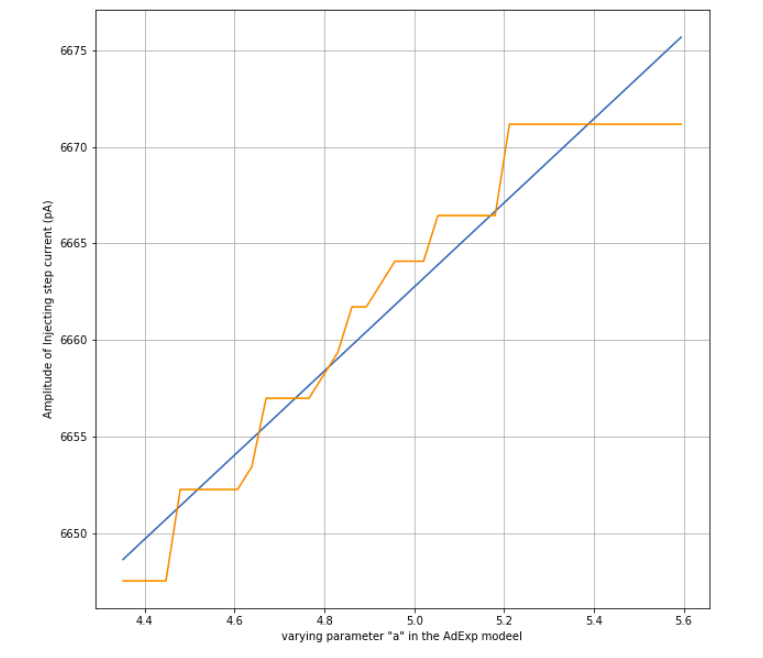
\includegraphics[]{figures/fundamental_cause_of_corrogations.png}
\caption[]{The main cause of corrugated error surfaces in this work was found to be re-calculating special current values on a per-model basis. In this plot, for each data point in blue and orange traces, the model was forced to fire exactly 11 spikes while the value of 'a' was swept between $4.4$-$5.6$, a straight line given by linear regression, approximates where we expect required current injection amplitude to fall, but instead, the real value routinely zig-zags to either side of the straight line. These deviations in current injection values represent a small but measurable amounts of excess currents. Current that was slightly more than sufficient to cause 11 spikes but less sufficient to cause 12 spikes. These current excesses are free to propagate into other measured features of spiking waveforms where they amplify a small but significant amount.

In the above discussion a hypothetical sceanario was described, where an optimizer measures ISIs at 1.5 $times$ rheobase, because the ISI measurement is contigent on Rheobase measurements, the rheobase approximation error is manifest in ISI too.}
\end{figure}
\end{center}

Below I show a more concrete example of the same phenomena.
\begin{figure}
\begin{center}
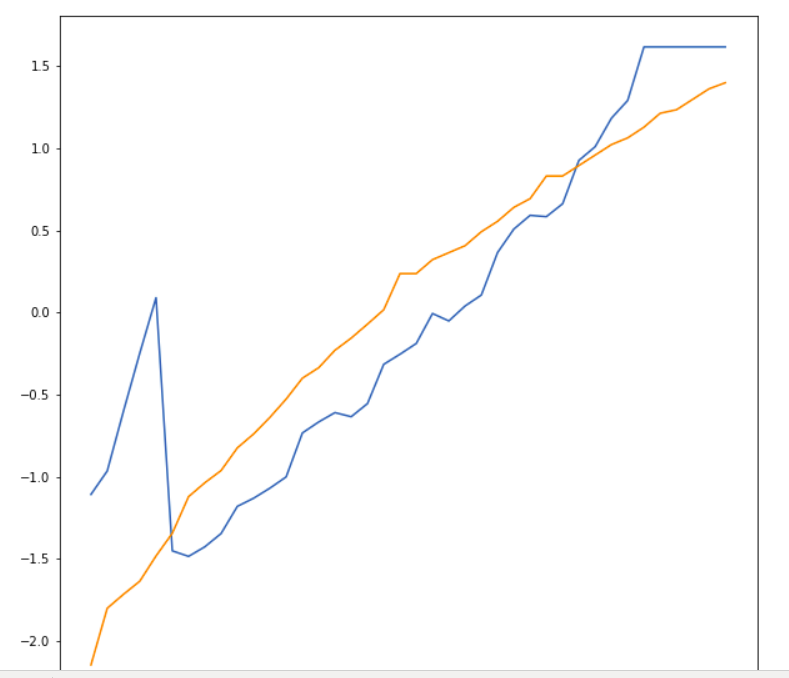
\includegraphics[]{figures/rh_vs_vt.png}
\caption{An izhikevich model is used to examine the effects of slowly varying parameter 'a' while keeping all other paramters as constant, on the plot, rheobase and $V_{T}$ are calculated for each different value of 'a' and plotted on the same y-axis. It becomes apparent that rheobase (the orange trace) has minor zig-zags in its value, while $V_{T}$, has bigger and more significant zig-zags in its value, at this point all we have done is slowly varied and calculated $V_{T}$ but we have not plotted $V_{T}$ in relation to APs}
\end{center}
\end{figure}

\begin{figure}
\begin{center}
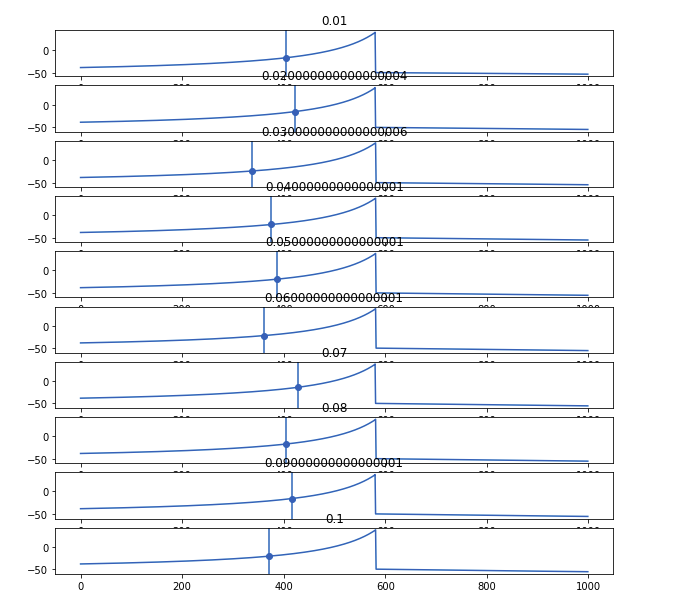
\includegraphics[]{figures/variable_vt.png}
\caption[Source of corrugation]{It is clear from the plot above, that $V_{T}$ zigzags in value unpredictably as we smoothly change the value of $'a'$ in the Izhikevich model, but we want to see if this oscillatory behavior is noticeable if we plot $V_{T}$ on AP waveforms, as we vary $'a'$. In the following plot made of inset figures. $'a'$ starts at $0.01$ in the top most figure, and slowly works its way up to $0.1$ in the bottom most figure. For each value of 'a' we calculate Rheobase, and then $V_{T}$ as $V_{T}$ is contingent. Unpredictably $V_{T}$ oscillates backwards and forwards, instead of consistently increasing or decreasing. In this way, I have shown how, small residual errors starting in necessary approximations of rheobase value, have moved into $V_{T}$ where they are slightly amplified, however, this just marks the beginning of the problem.  

AP amplitude measurements and AP width measurements happen to be contingent, on $V_{T}$, but the measured height and width are anchored to $V_{T}$ the very reading that we can see unduly oscillating back and forth. Therefore low amplitude oscillatory error is then introduced into spike height and spike width also.}
\label{fig:variable-vt}
\end{center}
\end{figure}

%An izhikevich model is used to examine the effects of sweeping across changes to parameter 'a' while retaining all other paramters as constant, on the plot, rheobase is and $V_{T}$ is calculated for each different value of 'a' and plotted on the same y-axis. It becomes apparent that rheobase (the orange trace) has minor zig-zags in its value, while $V_{T}$, has bigger and more significant zig-zags in its error, at this point all we have done is slowly varied and calculated $V_{T}$ but we have not plotted $V_{T}$ in relation to APs

% If all other conditions are favorable , as the remaining objective functions may have high fidelity; 

Since some care was taken to choose remaining error functions, optimization is still viable despite potentially misleading surface defects, because generally there is enough helpful information in the error surface to guide optimization.% these corrogated defects in error surface are not completely 

By necessity the rheobase determining algorithm utilized in this work has a finite precision. So although in theory rheobase is defined as the minimum current amplitude to cause exactly one spike, in practice there will be small variable amounts of excess current injection strength. Such propagating errors were applied to many threshold dependant waveform features. Its important to note that because resulting corrugations were smaller in amplitude than other important features of the error surface. Humans can conceptualize the small amplitude corrugations as noise. Optimization in the presence of such noise sources was often viable, but in such a case, successful optimization becomes contingent on the satisfaction of other favorable conditions





One solution is make tests depend on a static value of rheobase sourced directly from the experimental data, rather than using the rheobase which belongs uniquely to the current models parameter set.
In other words, if the rheobase of the biological neuron is 100 pA, then the $1.5\times$ rheobase ISI test should be performed with a current injection of 150 pA, even if the rheobase of the current model parameterization is some entirely different value.
In practice this is less costly than optimizing over an intractable, corrugated error surface.

%%
% No! I think this would exclude space quicker and therefore save time. it would not cost time.
%%%
%In principle, this means wasting a bit of extra computation time exploring some poorly-fitting parameter sets, but 

Another approach is to dispense with the rheobase entirely, and simply test using a fixed set of current amplitudes that span the suprathreshold portion of the F-I curve, e.g. 200pA, 350pA, and 500 pA for a typical neuron.
This seems extremely direct, but it in some cases it fails to explore the most interesting peri-threshold portion of the F-I curve, where the dynamics of single spikes contain a great deal of information about peri-threshold dynamics.
For example, an after-hyperpolarization that is visible after single spike at rheobase may become completely swamped by the combination of inward pipette current and sodium current at values of injected current that are high above threshold.

\subsection{Error Surfaces}
In methods I describe two approaches to fitting models, one of those approaches involved a supra-threshold virtual experiment that guides optimization, in models when more than one spike is measured. The other approach involves an at-threshold virtual experiment that guide optimization, where one or no spikes are expected.

It is important to know which approach resulted in the smoothest and most tractible error surfaces. Below I plot error surfaces from each kind of paradigm, such that the reader can also asses which surface look more useful for optimisation. 

Case 1, Izhikevich model at threshold virtual experiment. Constraints used:
\begin{tabular}{}c}
    TimeConstantTest \\
    RestingPotentialTest \\
    InputResistanceTest \\
    CapacitanceTest \\
    FITest \\
\end{tabular}

All the figures below employ a consistent color coding scheme where red encodes the highest error and blue the lowest error. Because the reduced neuronal models are high dimensional the easiest way to view the error surface the models experience under optimization is to make 2D plots of their surface for each different pairings of $12$ model parameters.

%The surface plot from the supra threshold paradigm shows more contrast for two reasons: 1, it has less intermediary values (light green colour), reason two, it less high frequency changes, or ripples in the error surface.  


\begin{figure}
    \centering
    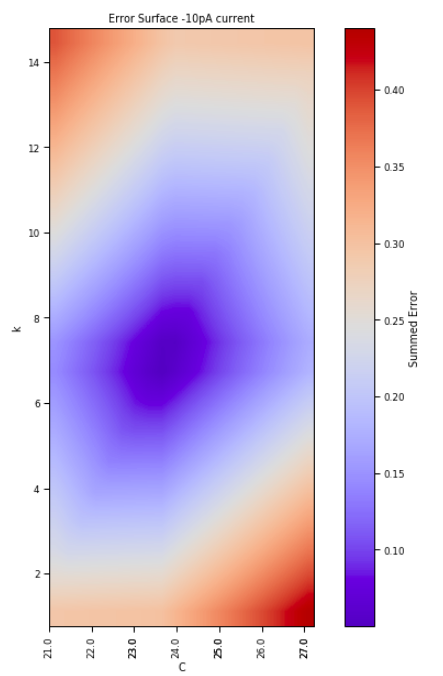
\includegraphics[scale=0.7]{figures/friendly_error_surface.png}
    \caption[Using only constant currents causes simple tractable error surfaces]{Because a constant current injection of $-10pA$ was applied, the error surface is simple informative and very easy to navigate, although only one slice into the error hypervolume is shown. Plots of GA learning speed provide also demonstrate that the error surface is free from both corrugation and discontinuity. Other plots (not shown here) demonstrate that all other slices into the hypervolume have simple convex shape.}
    \label{fig:constant_current}
\end{figure}


Case 2, AdExp Model model supra-threshold virtual experiment. Constraints used:
\begin{verbatim}
adaptation_index,
adaptation_index2 
time_to_first_spike, mean_AP_amplitude,
spike_half_width, 
AHP_depth,minimum_voltage,
peak_voltage,
time-to-last-spike,
AHP-depth-abs,
all_ISI_values
voltage_base, 
min_voltage_between_spikes,
Spikecount
 \end{verbatim}
\begin{figure}
    \centering
    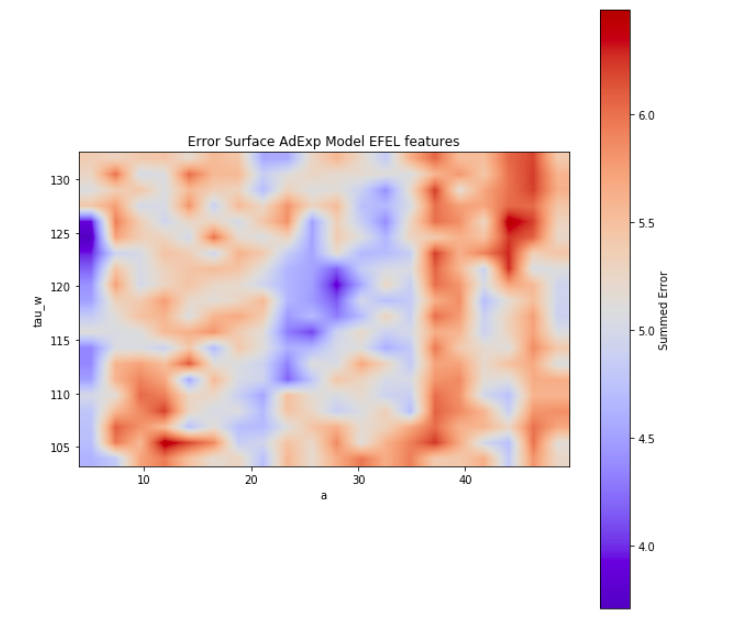
\includegraphics[scale=1.25]{figures/adexp_efel_problem.png}
    \caption[A very complicated but not hopeless error surfaces]{A two dimensional error surface drawn from summed EFEL error scores, acting on Adaptive Exponential models.
    
    The optima chosen by the optimizer was actually the one in the centre, and not the one on the left, bear in mind, however, that these are only two out of approximately 12 model dimensions, and these two dimensions may not have weighed heavily in the final summed score (as opposed to the component error depicted here)}
    \label{fig:real_problem_nontrivial_surface}
\end{figure}

\begin{figure}
    \centering
    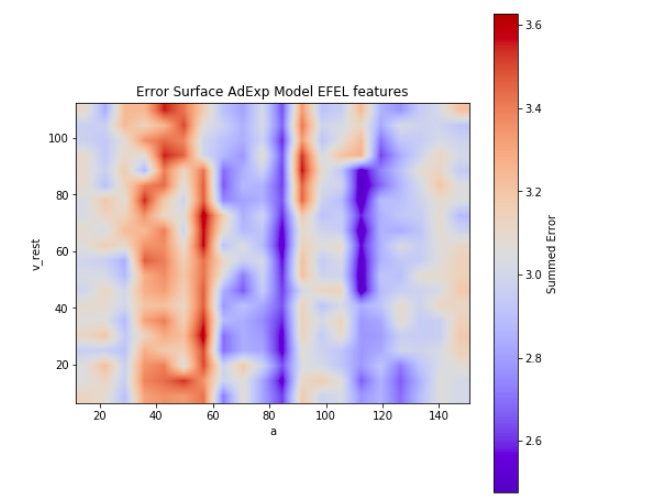
\includegraphics[scale=1.25]{figures/third_error_surface.png}
    %\caption[Cliff ledge in 2D error surface]{Cliff ledge in 2D error surface}
        \caption[Complex but not hopeless error surfaces]{Complex error surface with alternating neighbouring ridges and valleys (ripples)}
    \label{fig:real_problem_nontrivial_surface}
\end{figure}

I suspect that other pre-existing optimizers that fit neuronal models are largely ignorant of the error surface they face.
In fact, without comprehensive data about the convergence rates of various competing approaches to optimization, we cannot now how efficiently each obtains its solutions, nor about alternative solutions that may have been missed.

Nonetheless, I am confident that genetic algorithms (in general) are preferable to to exhaustive search (which is impractical for all but the smallest models) and to gradient-descent-like approaches (due to the nature of the error surface).
Unfortunately, efficient optimization often warrants a small cursory grid search of the parameter space, and this grid search introduces circularity back into methodology. What we wanted was a way to avoid the exhaustive search, and therefore the optimizer must be able to search autominously.
% NB, this is harder to understand than the residual rheobase error idea.    


% dont need to share complexity with reader.
%Although not shown here a third case is worth describing, as this third test combination achieved many useful results: Izhikevich model at threshold virtual experiment. Constraints used:
%\begin{verbatim}
%Case1 + RheobaseTest,
%\end{verbatim}
